\section{Simulation experiments}
\subsection{Experimental setup and evaluation criteria}
The dynamic simulator integrates the payload and every aircraft as free rigid bodies in MuJoCo~\cite{mujoco2012}. Individual rotor-site forces generate aircraft translation and rotation, and the cable law in Eq.~\eqref{eq:cable} generates the load reactions. Table~\ref{tab:parameters} summarizes the model and sensing settings. The default physical integration step is 0.5 ms, and motor commands are updated at 50 Hz. Computation is executed on a workstation with an AMD Ryzen 9 8945HX processor and an NVIDIA GeForce RTX 5070 Ti Laptop GPU.

\begin{table}[t]
\centering\small
\caption{Dynamic and sensing parameters. Noise bounds apply to the corresponding virtual measurements.}
\label{tab:parameters}
\begin{tabular}{@{}ll@{}}\toprule
Quantity & Value\\\midrule
Aircraft mass & 1.0 kg\\
Aircraft inertia diagonal & $[.009,.009,.016]$ kg m$^2$\\
Cable rest length & 2.0 m\\
Cable stiffness / damping & 180 N/m / 5 N s/m\\
Maximum thrust per motor & 7.5 N\\
Motor response time constant & 25 ms\\
Aircraft linear drag coefficient & 0.2 N s/m\\
Local ICP RMSE / inlier gate & 18 mm / 0.65\\
Correspondence gate & 80 mm\\
Control / RGB-D request rate & 50 Hz / 10 Hz\\
RGB-D image resolution & $256\times192$ pixels per view\\
Depth noise standard deviation & 1 mm\\
Tension noise & Uniform $\pm0.01$ N\\
Aircraft position noise & Uniform $\pm0.5$ mm\\
Preparation motion & 16 s\\
Physical integration step & 0.5 ms\\\bottomrule
\end{tabular}
\end{table}

Two complementary task groups are evaluated. The base group comprises rectangular and nonconvex stepped payloads, each carried by three and four aircraft, as illustrated in Fig.~\ref{fig:configurations}. Each configuration is paired with a uniform-shape control model, giving eight task attempts. Within each pair, the object, hidden ballast, sensor seed, preparation procedure and planning rules are held fixed. The uniform model distributes a nominal 1.05 kg over interior scan-support locations, while the identification model uses Eq.~\eqref{eq:fit}. The comparison therefore evaluates the inertial information supplied to planning and feedback under the same acquired external geometry.

\begin{figure*}[t]
\centering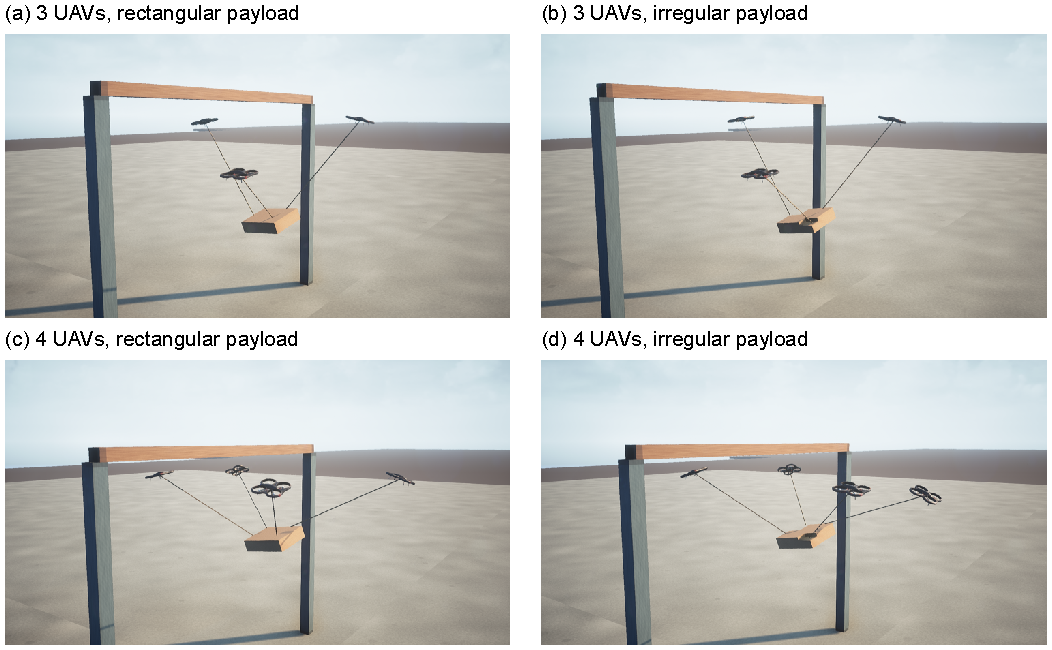
\includegraphics[width=.90\textwidth]{fig04_configurations.pdf}
\caption{Team-size and shape configurations in the base experiments. (a),(b) Three UAVs carrying rectangular and irregular payloads. (c),(d) The corresponding four-UAV configurations. All panels use original Unreal images of the recorded dynamic executions.}
\label{fig:configurations}
\end{figure*}

The second group carries a forked payload through sequential restrictions. The object measures $1.21\times0.90\times0.40$ m and has unequal side arms, open bays and a raised boss. Four mounts are installed at material-supported outer corners. Fixed padeyes, rotating shackles and rope terminations share the same attachment geometry as the force model. Mount mass and inertia are included in the load properties. The effective 2 m cable includes the 60 mm rigid termination, with the force application point at its pin center. These details permit large rotations while maintaining consistent visual and mechanical attachments.

Execution acceptance requires completed transport, peak position error at most 0.10 m, peak rotation error at most $5^\circ$, and tensions strictly between 0.5 and 9 N. Additional limits are $40^\circ$ aircraft tilt, 7.5 N per motor, 2.6 m/s aircraft speed and 6 m/s$^2$ aircraft acceleration. Rotation error is the magnitude of the logarithm of $RR_r^T$. Rigid-body contacts are monitored at physical substeps. Complete cable-segment checks use the 50 Hz records; the course clearance analysis inflates segment radius by the termination width and half a sampling interval of endpoint motion. Corresponding obstacle and load-body checks use the complete saved segment, rather than only cable endpoints.

The RGB-D inputs used for identification and feedback are rendered from the dynamic state and returned through the image-processing interface. Separately, Unreal Engine 5.2 and the CityPark Showcase environment produce the presentation images and videos. The distinction follows the useful separation between visual and physical simulation~\cite{airsim2017}: in this study numerical performance is measured from the MuJoCo closed loop, and Unreal displays those recorded states. The video output is $1920\times1080$ at 25 frames/s with one-to-one physical time. No display interpolation changes the recorded motion.

\subsection{Complete inertial identification and held-out prediction}
Across the four base configurations and two forked-payload executions, mass relative error is 0.0024--0.0188\%, and the CoM-inertia Frobenius relative error is 5.46--7.87\%. True and estimated mass, three-axis CoM, all six origin-inertia entries and principal moments are provided in the public numerical records. Figure~\ref{fig:identification}(a),(b) therefore evaluates the complete ten-parameter model rather than using CoM accuracy as a proxy for inertia accuracy. 
Figure~\ref{fig:identification} compares the models used for transportation. The identified CoM errors range from 0.39 to 2.18 mm across the four configurations. In contrast, the uniform-shape models differ from the actual CoM by approximately 103--117 mm. The external shape and installation coordinates are available to both models, so this difference concerns internal mass moments rather than surface acquisition.

Figure~\ref{fig:identification}(c) evaluates observation geometry at causal prefixes from 4 to 16 s. The normalized systems have rank ten, with condition numbers of approximately 4.4--9.0. At a 6 s prefix, the original activation criteria are satisfied in all four base cases. The prefix calculations share the original observation streams and quantify information availability during preparation.

For predictive evaluation, complete 0.4 s integral windows are formed from transport-only observations, excluding the first and last second of transport. These samples do not enter the preparation fit. Figure~\ref{fig:identification}(d) compares each model's predicted moment impulse against the true-inertia prediction on the same held-out regressor. Matching the uniform model's total mass isolates its remaining first- and second-moment errors. The repository also reports measured impulse residuals for both the fitted and true-inertia models, so parameter-model discrepancy can be distinguished from observation and integration residuals.

The completed four-aircraft rectangular pair provides a direct tracking comparison. Its uniform model has 102.75 mm CoM error and $22.05^\circ$ peak attitude error. With the identified model, these values are 0.39 mm and $0.66^\circ$. Peak translation error decreases from 8.19 to 2.76 cm. Thus the attitude error is reduced by approximately 97\% for this pair. The change has a mechanical explanation: a misplaced CoM creates an incorrect gravity moment in Eq.~\eqref{eq:moment}, which produces inappropriate cable-force distribution during rotation and load lowering.

\begin{figure*}[t]
\centering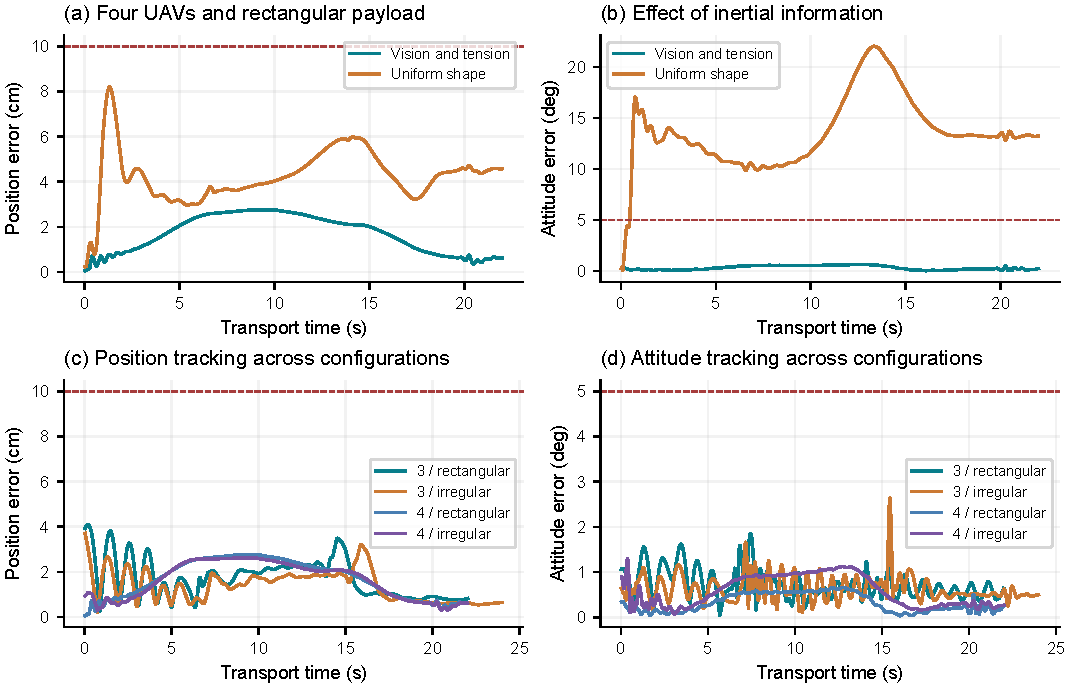
\includegraphics[width=\textwidth]{fig05_tracking.pdf}
\caption{Closed-loop tracking in the base experiments. (a),(b) Paired four-aircraft rectangular-payload executions with uniform-shape and identified inertial models. (c),(d) Identified-model position and rotation errors for all four team/shape configurations. Dashed lines mark the execution thresholds. Time is relative to each transport start.}
\label{fig:tracking}
\end{figure*}

\begin{table*}[t]
\centering\small
\caption{Base transport results with identified inertial moments. Each row is one executed team/shape configuration. Tension extrema include the complete preparation and transport at physical substeps.}
\label{tab:matrix}
\begin{tabular}{@{}clrrrrl@{}}\toprule
UAVs & Payload & Transport (s) & CoM error (mm) & Peak position (cm) & Peak attitude ($^\circ$) & Tension (N)\\\midrule
3 & Rectangular & 20 & 2.18 & 4.10 & 1.85 & 1.08--8.38 \\
3 & Irregular & 22 & 1.34 & 3.71 & 2.64 & 1.20--7.55 \\
4 & Rectangular & 20 & 0.39 & 2.76 & 0.66 & 1.63--8.69 \\
4 & Irregular & 20 & 0.68 & 2.62 & 1.29 & 1.03--8.61 
\\
\bottomrule\end{tabular}
\end{table*}

\subsection{Team size and payload geometry}
All four identified-model configurations satisfy the execution criteria. Table~\ref{tab:matrix} reports their individual results rather than treating them as repeated samples of one configuration. Peak position errors are 2.62--4.10 cm, and peak attitude errors are $0.66$--$2.64^\circ$. The three-aircraft irregular case selects 22 s from the candidate duration set; the other three use 20 s. Their peak payload speeds are 0.90--0.99 m/s, and average speeds within the central passage region are 0.84--0.93 m/s.

Figure~\ref{fig:tensions} shows cable loading during transportation. Across preparation and transport, tensions remain between 1.03 and 8.69 N. Aircraft, payload and cable-obstacle contacts are absent, and none of the identified-model runs saturates its motor commands. The four-aircraft rectangular formation reduces the vertical endpoint-to-payload envelope from a maximum of 1.94 m to a minimum of 1.09 m during the maneuver, while the endpoint lateral span varies between 1.86 and 3.38 m. The formation therefore changes the occupied vertical space by spreading the support directions as the payload passes beneath the beam.

\begin{figure*}[t]
\centering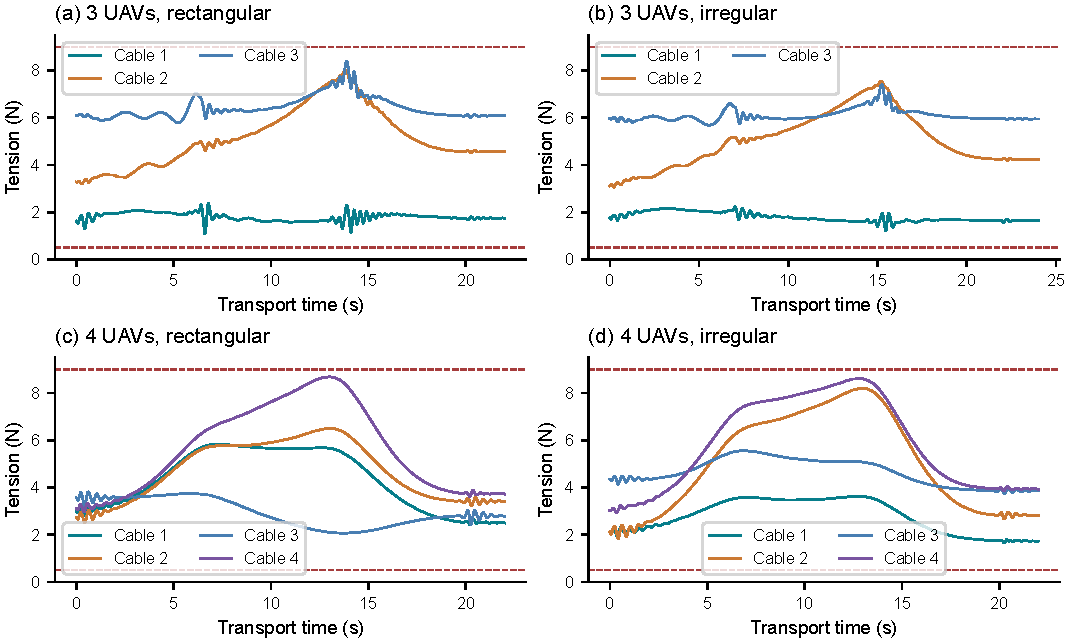
\includegraphics[width=\textwidth]{fig06_tensions.pdf}
\caption{Cable tensions during transport for the four identified-model configurations. Curves show 50 Hz saved states; dashed bounds are the 0.5--9 N execution limits. The extrema in Table~\ref{tab:matrix} additionally cover every physical substep and the preparation phase.}
\label{fig:tensions}
\end{figure*}

\begin{table*}[t]
\centering\small
\caption{Paired uniform-shape and identified-model outcomes under the same task rules. ``Planning rejection'' denotes that the candidate set did not produce an accepted force/geometry/actuation trajectory for that model.}
\label{tab:baseline}
\begin{tabular}{@{}clrlc@{}}\toprule
UAVs & Payload & Uniform CoM error (mm) & Uniform-model outcome & Identified outcome\\\midrule
3 & Rectangular & 103.35 & Planning rejection & Accepted \\
3 & Irregular & 115.31 & Planning rejection & Accepted \\
4 & Rectangular & 102.75 & Attitude limit exceeded & Accepted \\
4 & Irregular & 116.74 & Planning rejection & Accepted 
\\
\bottomrule\end{tabular}
\end{table*}

The uniform-model outcomes in Table~\ref{tab:baseline} complement the tracking example. Three configurations do not obtain an accepted candidate. The completed four-aircraft rectangular execution exceeds the attitude and aircraft acceleration limits. This comparison shows that the scanned outline alone does not provide the same task model as the outline augmented by measured inertial moments. Candidate rejection here is a result of the specified finite search, not a claim of global infeasibility of the physical task.

\subsection{Controlled ablations and sensor-seed repetitions}
The controlled comparison uses five inertial-information levels on each of the four base configurations: a uniform-shape model with true total mass; identified mass with uniform-shape CoM and central inertia; identified mass and CoM with mass-scaled uniform-shape central inertia; full identification; and true inertial parameters. All arms use the same acquired-geometry procedure, fixed ballast, sensor seed, preparation, reference family, candidate budget and feedback gains. The true-mass arm isolates errors in the first and second moments without a mass mismatch. The oracle is an information reference, rather than a competing planner.

\begin{table*}[t]
\centering\small
\caption{Five-arm controlled ablation. Entries give peak attitude error ($^\circ$) for completed executions. R denotes candidate planning rejection; A denotes an image-age abort before transport. Asterisks mark completed executions outside the common acceptance criteria. Each cell is one initial attempt, with all attempt records retained.}
\label{tab:ablation}
\begin{tabular}{@{}clrrrrr@{}}\toprule
UAVs & Payload & True mass, uniform & Mass only & Mass + CoM & Full identification & True inertia\\\midrule
3 & Rectangular & R & R & 1.75 & 1.81 & 1.80\\
3 & Irregular & R & R & A & 2.60 & 2.51\\
4 & Rectangular & 29.66\textsuperscript{*} & 29.44\textsuperscript{*} & 0.73 & 0.71 & 0.68\\
4 & Irregular & R & R & 1.16 & 1.06 & 1.14
\\
\bottomrule\end{tabular}
\end{table*}

Table~\ref{tab:ablation} distinguishes candidate availability from completed-transport accuracy. Both uniform-moment arms produce a candidate only for the four-aircraft rectangular configuration; its peak attitude errors are $29.66^\circ$ and $29.44^\circ$, respectively. All four full-identification and four true-inertia attempts satisfy the execution criteria. Three mass--CoM attempts complete and satisfy the criteria; the remaining acquisition abort is reported separately. In the four-aircraft rectangular case, their attitude peaks are $0.731^\circ$, $0.712^\circ$ and $0.678^\circ$. The dominant tracking gain in this task therefore follows CoM correction. The incremental effect of identifying central inertia is smaller and depends on the configuration; the three-aircraft rectangular mass--CoM arm, for example, has a slightly smaller attitude peak than its full-identification counterpart. Complete-inertia accuracy is assessed separately by Fig.~\ref{fig:identification} and transport-only prediction.

The three-aircraft irregular mass--CoM initial attempt stops on the image-age gate before transport and is retained as A, rather than classified as planning rejection. A separately labeled acquisition retry completes the task with a $2.54^\circ$ attitude peak. It does not replace the original table entry.

Twenty additional initial attempts use independent virtual sensor seeds for the fixed four-aircraft rectangular task. All 20 obtain an initial plan; 16 complete and satisfy the execution criteria, while 4 stop on the image-age gate. The all-attempt completion-and-acceptance rate is 16/20 (80\%; Wilson 95\% interval 58.4--91.9\%). Among the 16 complete transports, peak attitude error is $0.606$--$0.851^\circ$, and its median is $0.725^\circ$. Transport-only position RMS has median 1.96 cm and p95 1.97 cm; attitude RMS has median $0.427^\circ$ and p95 $0.488^\circ$. Initial planning time among complete transports has median 1.84 s and p95 1.89 s. These distributions are conditional on completed transport, and the initial attempts remain the statistical cohort even when a separately labeled diagnostic retry is available. The repeated task fixes shape and ballast; its seed distribution concerns sensing and acquisition timing under that configuration.

\subsection{Observation and support-model sensitivity}
Two archived preparation records, the four-aircraft rectangular case and the large-angle forked case, are each refitted under four declared measurement perturbations and twenty seeds per perturbation. The 160 fits isolate added pose noise (2 mm translation and $0.15^\circ$ rotation standard deviations), tension noise and bias (0.02 N each), fixed pose-frame bias (3 mm and $0.1^\circ$), and random observation removal (20\%). These synthetic ranges define a record-space sensitivity analysis; they do not represent hardware calibration or newly executed occluded-image flights. For the forked case, CoM-error p95 is 4.76 mm with added pose noise, 5.50 mm with tension perturbation, 2.25 mm with frame bias and 0.89 mm with observation removal. The corresponding central-inertia error p95 values are 19.52\%, 14.56\%, 11.05\% and 11.60\%. The full distributions for both records are available with the analysis protocol.

Changing $\lambda$ from $10^{-10}$ through $10^{-8}$ and $10^{-6}$ to $10^{-4}$ across all six nominal records changes CoM-error norms by at most 0.038 mm and central-inertia relative errors by at most 0.092 percentage points. A separate post-execution diagnostic restricts support locations to the evaluator's occupied body material for the two forked records. Central-inertia errors become 5.85\% and 6.72\%, compared with 5.86\% and 6.77\% for the acquired-surface hull. This comparison tests the moment envelope under the same observed motion; evaluator material geometry is used only in this diagnostic.

\subsection{Sequential apertures and large-angle reorientation}
The course comprises a 28 m centerline and twelve oriented solid obstacles: a laterally offset narrow frame, a low ceiling, a tilted frame, and three staggered blocks along the approach and exit regions. Figure~\ref{fig:course} shows the actual load and aircraft trajectories relative to these obstacles. Two course executions use the same forked object and corner mounts. The moderate-rotation course has a 2.70 m first opening and an 85 s transport. The large-rotation course narrows this opening to 2.10 m and uses a 125 s transport. The ceiling underside is 4.45 m above the ground, and the tilted opening has 2.85 m clear width.

\begin{figure*}[t]
\centering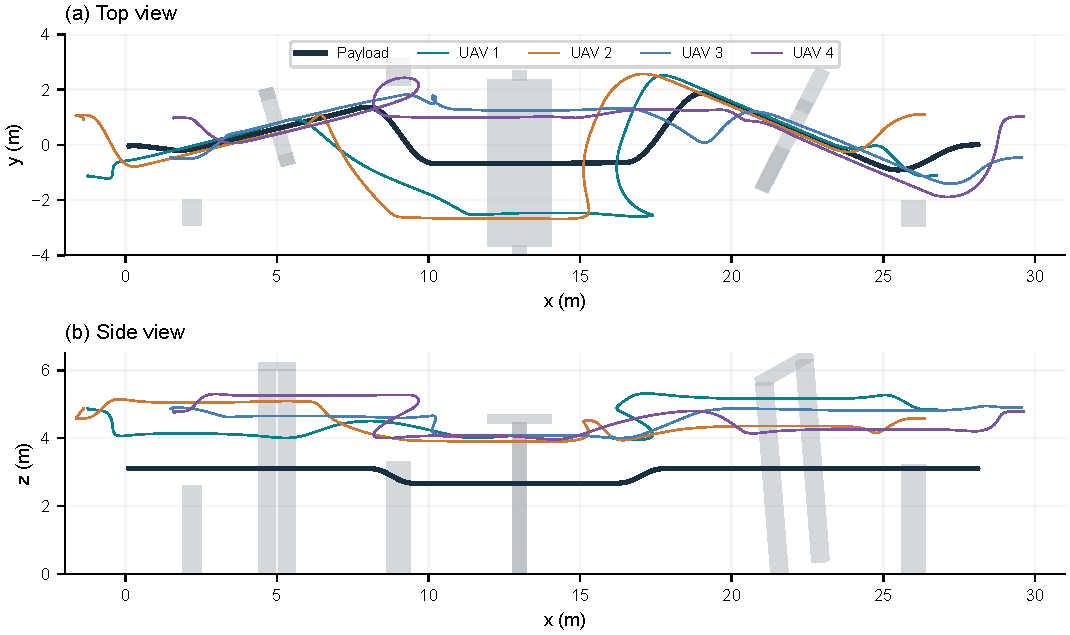
\includegraphics[width=\textwidth]{fig07_course.pdf}
\caption{Actual large-rotation course trajectories in (a) top and (b) side views. Gray polygons are projections of the twelve oriented obstacle boxes. The payload centerline and all four aircraft centers are plotted from the same dynamic execution.}
\label{fig:course}
\end{figure*}

In the large-rotation execution, the load is nearly horizontal at the start, rotates side-on for the first frame, returns to horizontal while changing heading under the ceiling, and rolls toward the opposite side for the last opening. Figure~\ref{fig:overview}(a)--(c) displays the three crossing configurations. The actual roll ranges from $-86.64^\circ$ to $90.34^\circ$, and yaw ranges from $-25.25^\circ$ to $90.85^\circ$. At the three crossing instants the roll angles are $90.03^\circ$, $0.03^\circ$ and $-84.24^\circ$. These rotations are achieved through cable loading while the team progresses along the course.

Figure~\ref{fig:course_dynamics} relates these attitudes to the supporting formation. The maximum vertical aircraft span is 1.37 m; it falls to approximately 0.19 m at the low-ceiling crossing. The minimum inter-aircraft separation over the complete execution is 0.640 m. The formation is consequently layered during side-on support and flattened under the ceiling. Payload attitude, relative aircraft position and available space change together.

\begin{table*}[t]
\centering\small
\caption{Forked-payload course executions. The two tasks have different first-aperture widths and prescribed rotation amplitudes; each is evaluated against the common execution criteria.}
\label{tab:course}
\begin{tabular}{@{}lrrrlrr@{}}\toprule
Course & Transport (s) & Peak position (cm) & Peak attitude ($^\circ$) & Tension (N) & Min. separation (m) & Planning (s)\\\midrule
Moderate rotation & 85 & 4.06 & 1.73 & 2.11--4.89 & 0.946 & 14.69 \\
Large rotation & 125 & 3.34 & 2.19 & 2.11--4.75 & 0.640 & 24.85 
\\
\bottomrule\end{tabular}
\end{table*}

Table~\ref{tab:course} reports the course results. The large-rotation execution has a 3.34 cm peak position error and $2.19^\circ$ peak attitude error. Tensions remain between 2.11 and 4.75 N, maximum aircraft tilt is $16.13^\circ$, and maximum aircraft speed is 2.38 m/s. The actual payload peak speed is 1.05 m/s. There are no rigid-body contacts, sampled cable-obstacle or cable-body intersections, slack cables or motor saturation intervals. All 1682 processed visual observations are valid under the registration tests.

The large-rotation geometric audit finds 0.081 m minimum aircraft clearance after a 0.28 m envelope inflation and 0.268 m minimum scanned-surface clearance after 0.045 m inflation. Complete cable segments are checked with a 0.0468 m radius including termination width and observed half-sample motion. These are sampled geometric margins with the stated motion inflation; they are not a general continuous-time safety certificate under arbitrary execution disturbances. The corner attachment geometry remains outside the material body during rotation. The full physical task takes 169.58 s, including 16 s preparation, identification and planning waits, transport, and terminal holding.

\begin{figure*}[t]
\centering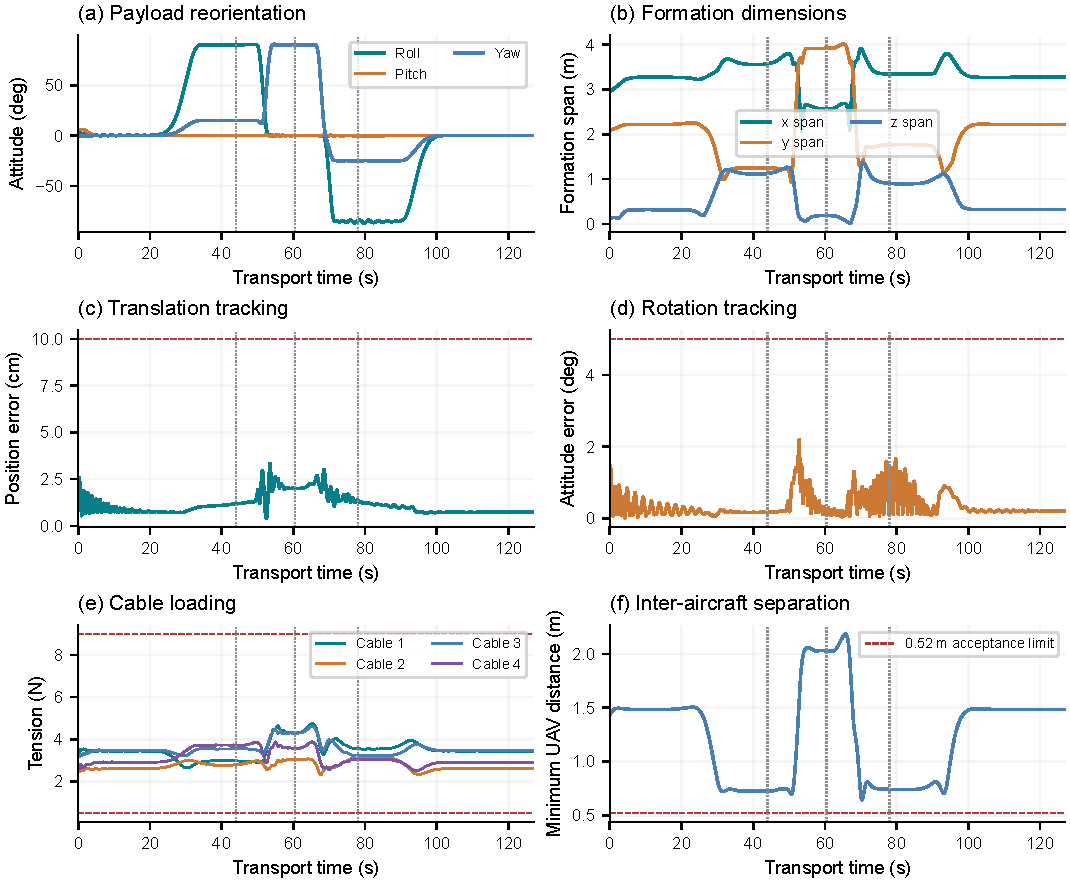
\includegraphics[width=\textwidth]{fig08_course_dynamics.pdf}
\caption{Large-rotation course dynamics. (a) Payload attitude. (b) Aircraft center span along each axis. (c),(d) Position and rotation errors. (e) Cable tensions. (f) Minimum pairwise aircraft center distance. Dotted vertical lines indicate the three payload crossing instants. Dashed horizontal lines indicate the corresponding execution or separation thresholds.}
\label{fig:course_dynamics}
\end{figure*}

\begin{figure*}[!t]
\centering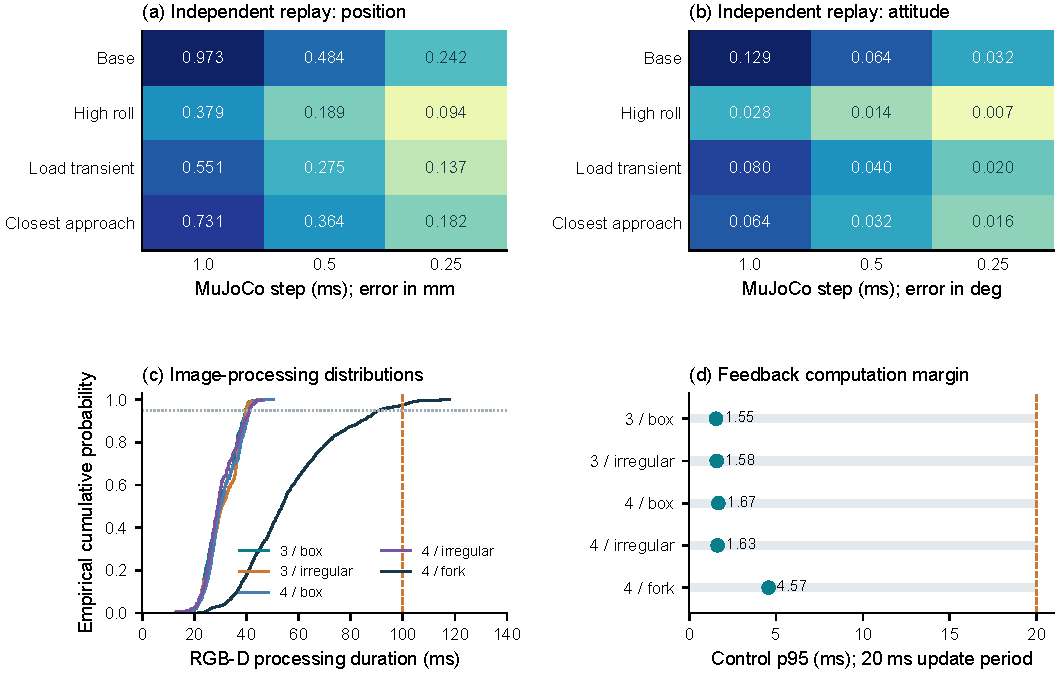
\includegraphics[width=\textwidth]{fig09_validation.pdf}
\caption{Numerical verification and computation distributions. (a),(b) Maximum payload CoM and attitude differences from independent two-second RK4 motor-command replay at three MuJoCo steps, including the base interval and three mechanically demanding course intervals. (c) Empirical cumulative distributions from all archived image-processing durations; the dashed vertical line marks the 100 ms RGB-D request interval. (d) Control-computation p95 values relative to the 20 ms control period. The separate computation paths do not imply 50 Hz image registration or whole-segment replanning.}
\label{fig:validation}
\end{figure*}

\subsection{Computation and numerical cross-checks}
For the four base identified-model configurations, initial whole-segment planning takes 0.74--1.56 s. Image processing p95 is 39.7--41.3 ms, control computation p95 is 1.55--1.67 ms, and sensor age p95 is 120--140 ms. The larger course requires additional conic separation updates and full-surface checks. Its initial plan takes 24.85 s, image processing p95 is 91.03 ms and control computation p95 is 4.57 ms. The observations remain asynchronous, with sensor age p95 of 160 ms. These timings separate pretransport trajectory construction from visual processing and feedback during motion. Force planning uses Clarabel with feasibility tolerance $2\times10^{-8}$, absolute and relative gap tolerances $10^{-7}$, and at most 100 iterations. Moment fitting uses feasibility tolerance $10^{-9}$ and absolute gap tolerance $10^{-10}$. The archived solver diagnostics retain the iteration counts for individual candidates.

Numerical consistency is examined using a two-second interval from the three-aircraft irregular-payload base execution, starting at physical time 29.30 s. A separately coded NumPy rigid-body model integrates the recorded motor inputs with fourth-order Runge--Kutta at 0.25 ms, without resetting the state inside the interval. As the MuJoCo step decreases from 1 to 0.5 and 0.25 ms, the maximum payload CoM difference decreases from 0.973 to 0.484 and 0.242 mm. The corresponding rotation differences are $0.1291^\circ$, $0.0642^\circ$ and $0.0320^\circ$; aircraft CoM differences decrease from 3.468 to 1.727 and 0.862 mm. Figure~\ref{fig:validation}(a),(b) includes this interval together with three additional two-second intervals from the large-angle course: maximum absolute roll, maximum sampled tension variation, and minimum aircraft-envelope clearance. Each interval is replayed continuously without interior state resets. At a 0.5 ms MuJoCo step, the added intervals differ from the independent RK4 replay by at most 0.365 mm in payload CoM and $0.040^\circ$ in attitude; halving the step approximately halves these differences.

A complete closed-loop rerun of that base configuration at a 0.25 ms step also satisfies the execution criteria, with 3.53 cm peak position error, $2.59^\circ$ peak attitude error and 1.20--7.53 N cable tensions. Together, the interval comparison and refined closed-loop execution examine both the numerical force implementation and the resulting feedback trajectory.



\subsection{Implications for cooperative transport}
The experiments connect three different kinds of information. The scan supplies the object's occupied geometry and a consistent frame for calibrated attachments. Tension and motion reveal the mass moments needed to balance and rotate that object. The force-to-endpoint map then converts the identified mechanics into aircraft geometry. The paired base experiment quantifies the effect of supplying those moments, while the sequential-aperture experiment shows how compliant support geometry changes during substantial load rotation.

The evaluated configuration uses calibrated external virtual RGB-D views, static payload mass distributions and known obstacle geometry. These conditions define the sensing and task model of the reported experiments. An onboard implementation introduces camera occlusion, calibration drift and different image coverage; changing payload contents introduces time-varying inertial parameters. These extensions call for corresponding sensing and replanning mechanisms. Within the evaluated setting, the current results establish continuous large-angle closed-loop transport across the specified apertures, with explicit load, cable and aircraft measurements.
